%%%%%%%%%%%%%%%%%%%%%%%%%%%%%%%%%%%%%%%%%%%%%%%%%%%%%%%%%%%%%%%%%%%%%%%%
\documentclass[twoside,uplatex]{ujarticle}
% 学部指定のフォーマットに近づける
\usepackage{jcis}
\usepackage[deluxe]{otf}

\usepackage[dvipdfmx]{graphicx}
% 他のパッケージ・スタイルを使う場合には適宜追加


%%%%%%%%%%%%%%%%%%%%%%%%%%%%%%%%%%%%%%%%%%%%%%%%%%%%%%%%%%%%%%%%%%%%%%%%
%% 論文著者記入項目 %%%%%%%%%%%%%%%%%%%%%%%%%%%%%%%%%%%%%%%%%%%%%%%%%%%%
%%%%%%%%%%%%%%%%%%%%%%%%%%%%%%%%%%%%%%%%%%%%%%%%%%%%%%%%%%%%%%%%%%%%%%%%

%% 表題
\title{卒業研究のありかたと、その発表様式の考察}

%% 副題 (副題がなければ空欄にする)
\subtitle{--- 形式面での実例として(本文約1280字)---}

%% 学籍番号 \studentID
\studentID{1108XX0000}

%% 著者名 \author
\author{文情 太郎}

%% 主担当 \mainAdviser
\mainAdviser{新島 襄 教授}

%% 副担当 \subAdviser (三名まで記述可)
% (注) 副担当は最大三名まで指定可能.
%      副担当が一人の場合は \subAdviserSecond{null},\subAdviserThird{
%      null} とする.
%      副担当が二人の場合は \subAdviserThird{null} とする.
\subAdviserFirst{新島 八重 教授}
\subAdviserSecond{null}
\subAdviserThird{null}

\begin{document}

%%%%%%%%%%%%%%%%%%%%%%%%%%%%%%%%%%%%%%%%%%%%%%%%%%%%%%%%%%%%%%%%%%%%%%%%
%% 表題・副題・学籍番号・著者名・主担当・副担当 表示
\maketitle
%% 引用していない参考文献も全部表示
\nocite{*}
%%%%%%%%%%%%%%%%%%%%%%%%%%%%%%%%%%%%%%%%%%%%%%%%%%%%%%%%%%%%%%%%%%%%%%%%
%% 本文 %%%%%%%%%%%%%%%%%%%%%%%%%%%%%%%%%%%%%%%%%%%%%%%%%%%%%%%%%%%%%%%%
%%%%%%%%%%%%%%%%%%%%%%%%%%%%%%%%%%%%%%%%%%%%%%%%%%%%%%%%%%%%%%%%%%%%%%%%

\section{はじめに}
卒業研究のありかたは適宜指導され、またその結果発表の様式はwebに公示され
ている。本研究は、その理念像を探索し、UML による卒業研究全体像を構築する
。そして、その枠組みにおいて卒業研究がどのように行われるべきであり、その
成果をどのように公表すべきかを考察することを目的とする。


\section{先行研究}
先行研究としては、実学の面からは「論文の書き方」の類が想定される。また枠
組みの設定としては、コンピュータなどが存在しない時代の考え方ではあるにせ
よ、ドイツ観念論から借用することもありうる。先行研究を探索することは重要
であり、手短に纏めておくことも必要ではあるが、最も重要なのは自分自身が研
究した部分であるということが理解されていなければならない。


\section{分析(あるいは解析)}
\subsection{分析データ(解析対象データ)}
データとはそもそも何かを考えることも重要である。しかし、考えただけでデー
タが取得できていないのでは仕方ない。課題に従ってデータの範疇は設定される
。量的データ、質的データを適切に収集する必要がある。また、構造を読み解い
て何らかのダイアグラムとするにあたっても、適切な原因・結果関係を提示せね
ばならない。まずもって、分析に値するデータの取得が必要である。

分析対象として『2008年度某学科卒業論文概要集』をとり、構成が適切か、結果
が明示されているかなどをデータ化した。


\subsection{分析方法}
データサイエンスにおける分析手法は多様である。データサイエンス(あるいは
文化情報学)という用語そのものは内包的あるいは外延的に固定して規定される
ものではなく、時代とともに進化し発展する。文化情報学は文理融合な学際的学
問であり、その立ち位置は揺らがなくとも実質内容は常に変化している。化石の
ように固定されているものではない(化石ですらその同定・分類もまた学説の進
歩とともに変化する)。しかし、「データに語らせる」という基本理念は保たれ
る。その為には、正しいデータの設定が必要であるのは当然であり、統計学的処
理等を誤って適用すればそれはデータを損なう行為である。

従って、データの科学的処理が必要であり、また処理結果の正しい解釈が必要と
なる。処理においては、何度もデータ様式を変更してやりなおすことが屡々起こ
るので、操作しやすく、またその処理内容が理解できるソフトウェアが好ましい
。

さらに、分析・解釈において用語や理論の不十分な理解で濫用すると(所謂「フ
ァッショナブル・ナンセンス」)、論文としての価値が認められない。


\subsection{分析結果}
『2008年度某学科卒業論文概要集』を分析した結果、よく構成されており研究の
価値が認められるものがある一方では、概要をみるかぎりでは何をしたのか全く
不明確なものもあった。そこで卒業論文本体と照合してみると、概要のレベルと
本体のレベルに有意な相関があると検定された。
検定のみではデータ全体像の把握に十分ではないので、さらに様々な処理と可視
化を行った。

\begin{figure}[htb]
 \centering
 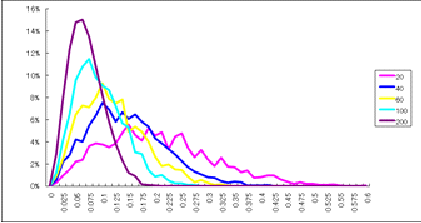
\includegraphics[width=7cm,clip]{sample.pdf}
 \caption{卒業論文レベルの減衰率分布}
 \label{fig:sample}
\end{figure}

\section{考察}
分野によって、考察を分析に組み込む場合もあり、またさらに別立てで「討論」
を記載する場合もある。これは分野ごとの常識に従っている。


\section{おわりに}
真面目な努力をしてきちんとしたデータの収集に努めたかどうか、正しい解析(
分析と解釈)を行ったかどうかが卒業論文で露わになると認める。


%%%%%%%%%%%%%%%%%%%%%%%%%%%%%%%%%%%%%%%%%%%%%%%%%%%%%%%%%%%%%%%%%%%%%%%%
%% 参考文献 %%%%%%%%%%%%%%%%%%%%%%%%%%%%%%%%%%%%%%%%%%%%%%%%%%%%%%%%%%%%
%%%%%%%%%%%%%%%%%%%%%%%%%%%%%%%%%%%%%%%%%%%%%%%%%%%%%%%%%%%%%%%%%%%%%%%%
\bibliographystyle{cis_abstract.bst} % cis_abstract.bst を利用
%\nocite{*}
\bibliography{sample}  % 作成した bib ファイルのファイル名を指定

\end{document}
